\chapter{Description des cas d'utilisation}
\label{s:Description_Utilisation}



\section{Diagramme des cas d'utilisation}

\begin{figure}[htp]
\centering
	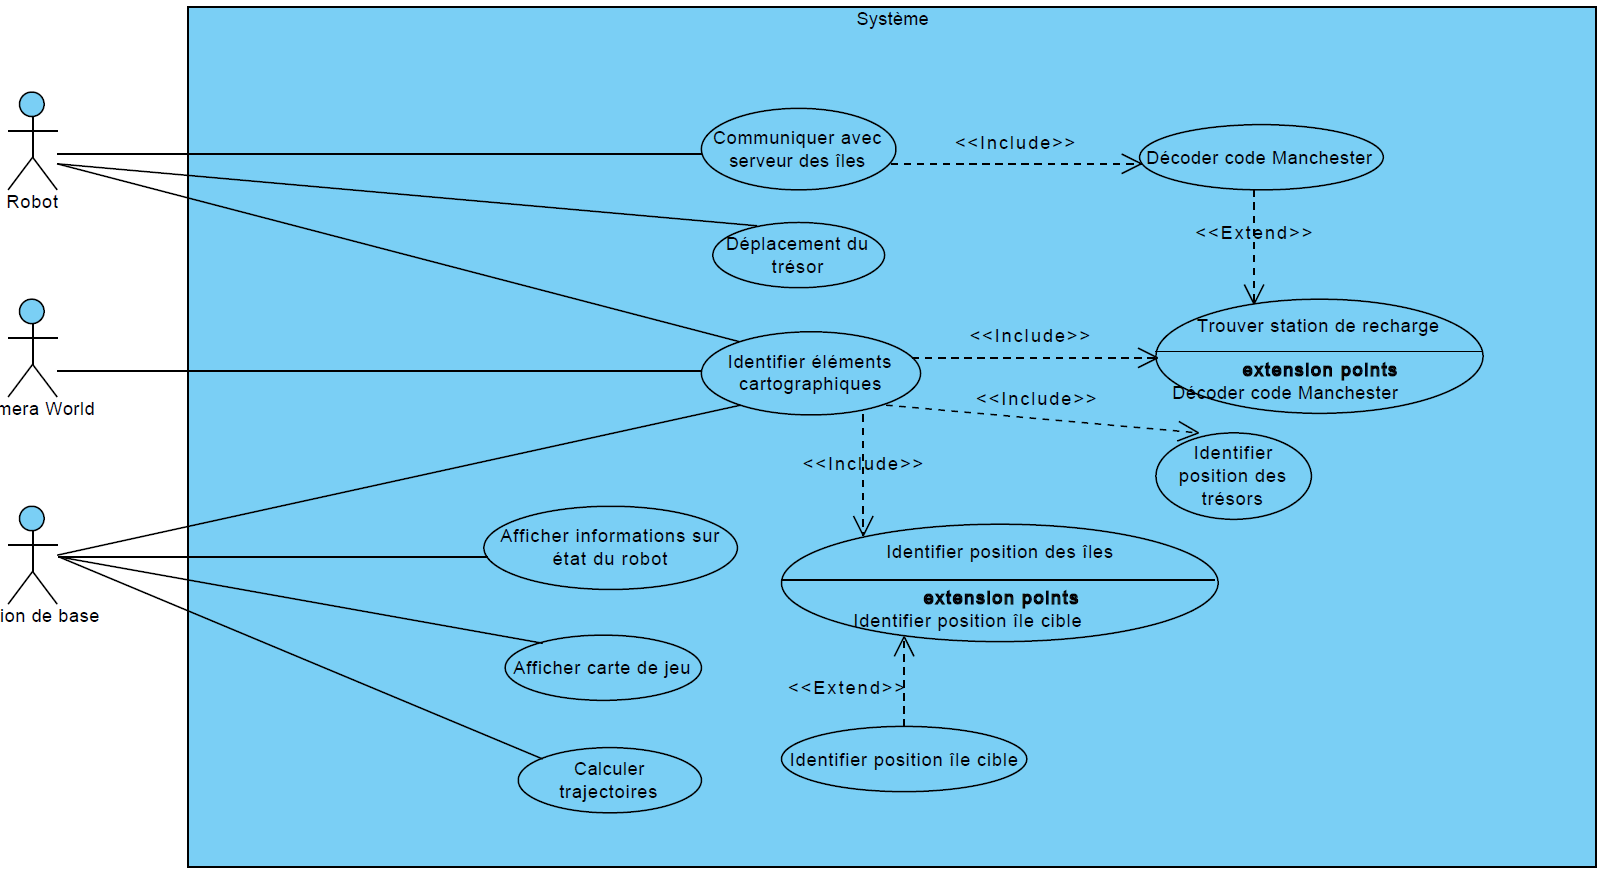
\includegraphics[width = 0.8\textwidth]{fig/casutilisation.png}
	\label{fig:Cas_Utilisation}
	\caption{Diagramme des cas d'utilisation}
\end{figure}


\pagebreak


\section{Sc�narios des cas d'utilisation}
%%%%%%%%%%%%%%% CAS UTILISATION 1 %%%%%%%%%%%%%%%%%
	%%%%%%%%%%% Identifier les �l�ments cartographiques  %%%%%%%%%%%%%
	%%%%%%%%%%%%% ETAT: A COMPLETER %%%%%%%%%%%%%%%%%%%%%%
    \begin{table}[!ht]
    \caption{Cas d'utilisation - Identifier les �l�ments cartographiques}
    \begin{tabular}{| l | p{4.75cm} p{4.75cm} |}
    \hline
    Cas d'utilisation & \multicolumn{2}{p{9.5cm} |}{Identifier les �l�ments cartographiques} \\ \hline
    Syst�me & \multicolumn{2}{p{9.5cm} |}{Syst�me de reconnaissance visuelle}\\ \hline
    Acteurs & \multicolumn{2}{p{9.5cm} |}{Robot, cam�ra world, station de base}\\ \hline
    Partie prenante et int�r�t & \multicolumn{2}{p{9.5cm} |}{Station de base : Vouloir identifier les �l�ments pr�sents sur la carte afin que le robot puisse remplir son mandat.}\\ 
    \hline
    Pr�conditions & \multicolumn{2}{p{9.5cm} |}{Le robot et la cam�ra world doivent fournir des images � la station de base}\\ \hline
    Garantie en cas de succ�s & \multicolumn{2}{p{9.5cm} |}{Les �l�ments cartographiques sont affich�s sur la carte de la station de base}\\ \hline
    
    \multirow{4}{*}{Sc�nario principal} 
    
    & 1. Big show baby & \\
    & & 2. Big show 2 baby \\
    & & 3.  Showtime \\
    & 4. Uiuuu & \\
    
    \hline
    
    \multirow{1}{*}{Sc�narios alternatifs} 
    
    & Aucun sc�nario alternatif & \\
    
    \hline
    \end{tabular}
    \label{tab:identifier_elements_cartes}
    \end{table}
    
    
%%%%%%%%%%%%%%% CAS UTILISATION 2 %%%%%%%%%%%%%%%%%
	%%%%%%%%%%% Trouver station de recharge  %%%%%%%%%%%%%
	%%%%%%%%%%%%% ETAT: A COMPLETER %%%%%%%%%%%%%%%%%%%%%%
    \begin{table}[!ht]
    \caption{Cas d'utilisation - Trouver la station de recharge}
    \begin{tabular}{| l | p{4.75cm} p{4.75cm} |}
    \hline
    Cas d'utilisation & \multicolumn{2}{p{9.5cm} |}{Trouver station de recharge} \\ \hline
    Syst�me & \multicolumn{2}{p{9.5cm} |}{Syst�me de reconnaissance visuelle}\\ \hline
    Acteurs & \multicolumn{2}{p{9.5cm} |}{Robot, cam�ra world, station de base}\\ \hline
    Partie prenante et int�r�t & \multicolumn{2}{p{9.5cm} |}{Robot : Faire le plein d'�nergie et recevoir le code Manchester}\\ 
    \hline
    Pr�conditions & \multicolumn{2}{p{9.5cm} |}{La station de base a identifi� la position de la station de recharge et une trajectoire a �t� calcul�e}\\ \hline
    Garantie en cas de succ�s & \multicolumn{2}{p{9.5cm} |}{La trajectoire menant le robot jusqu'� la station de recharge est affich�e sur la station de base. Le robot se d�place vers la station de recharge sans toucher � aucun obstacle.}\\ \hline
    
    \multirow{4}{*}{Sc�nario principal} 
    
    & 1. Big show baby & \\
    & & 2. Big show 2 baby \\
    & & 3.  Showtime \\
    & 4. Uiuuu & \\
    
    \hline
    
    \multirow{1}{*}{Sc�narios alternatifs} 
    
    & Aucun sc�nario alternatif & \\
    
    \hline
    \end{tabular}
    \label{tab:trouver_station_recharge}
    \end{table}


